\section{Security of the pipeline}
Security of the pipeline in the short term is the security measures that are taken into consideration when securing the pipeline itself. This includes not only securing the pipeline itself but also the infrastructure, components, and network that are used to process the code that goes through the pipeline. Securing the pipeline ensures that the code is not tampered with during the process of going through the pipeline. 


\subsection{Branch Protection}
\label{branchprotection}
Branch protection is a feature of GitHub, that enforces different rules and requirements for specific branches in the repository. The purpose of branch protection is to maintain the stability and security of the code, this is done by ensuring that all changes done to the branch have gone through the proper steps before being merged into the main codebase. Below are the different branch protection features that can be enabled in GitHub. \cite{ProtectedBranches}
\\
\subsubsection{Require a pull request before merging}
Administrators of the repository can add rules to the repository which restrict pull requests to have a specific number of people approving the changes before merging to a protected branch. Administrators can allow users with written permissions to do the approving as well as users considered to be code owners. 

It is under this type of protection that the "four eyes" principle is applied. Since this type of protection require that at least two people approve the merge, this includes the person itself doing the changes, this principle is a controlling mechanism that increases the security measures. 
\\
\subsubsection{Require status checks to pass before merging}
When users work together in the same repository, it is important to maintain the high quality of the code that's being pushed and merged. Enabling "require status checks to pass before merging" allow the administrators of the repository to set certain criteria that need to be fulfilled before the code is merged. 

\subsubsection{Require conversation resolution before merging}
When working together on the same repository it is important to have clear communication and collaboration  A way to secure this is to enable "require conversation resolution before merging". This allows all discussions regarding for example issues or pull requests that need to be properly resolved before any merging happens. 
\\
\subsubsection{Require signed commits}
Enabling require signed commits can be considered a security measure that secures that changes in the code have not been tampered with. 
To be able to have secured signed commits, all commits pushed to the repository must be signed with a \acrlong{gpg} key. A \acrshort{gpg} key is a unique digital signature that in short terms verifies the person that is committing to the repository is who they say they are. 


\subsubsection{Require linear history}
When enabling this security feature, it ensures that all changes done in the repository are done in a specific order, one after another without creating any branches or forks. This will as a result make it easier to keep track of all the changes that have been done and minimizes the chances of mistakes. Enforcing such measures restricts users from merging their changes with the main branch. 

\subsubsection{Require deployments to succeed before merging}
Require deployments to succeed before merging is another feature in GitHub, that allows the users to enforce that different required checks that have been created, such as pre-merge checks or automated tests, are passed before a pull request can be merged into the main branch.


\subsubsection{Lock branch}
Lock branch as the name implies allows the users to lock a branch in a repository, which will prevent changes from being made to the branch. This can be useful if there are situations where the branch needs to be protected from unauthorized changes or to be deleted. 


\subsubsection{Do not allow bypassing the above settings}
This feature, in short, prevents users in a repository from bypassing required checks that have been created or other restrictions. For example, if a user with admin access has configured a branch protection rule which requires that all pull requests reviews and status checks needs to be passed before merging, enabling this feature will then tell the user to go through these reviews and checks before any changes are done directly to the branch. 

\vspace{2mm}
\begin{figure}[H]
    \centering
    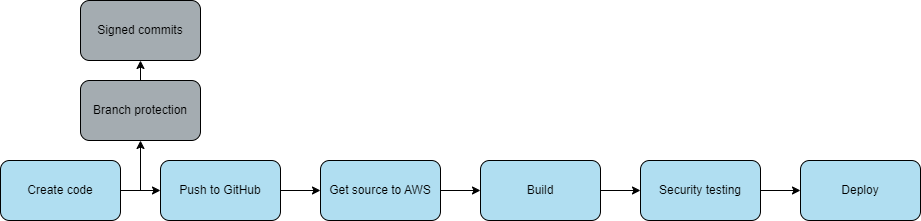
\includegraphics[width=0.8\columnwidth]{Images/pipeline6.png}
    \caption{Pipeline with implemented branch protection rules}
    \label{fig: Pipeline with implemented branch protection rules}
\end{figure}

\subsection{Access Control}
Access control involves implementing measures to regulate the individuals who are allowed to access certain resources like GitHub, as well as determining the appropriate level of access for each individual. When applying these measures, one should follow the "least privilege" principle. According to NIST, this is \textit{"the principle that a security architecture should be designed so that each entity is granted the minimum system resources and authorizations that the entity needs to perform its function"}\cite{leastprivilege}. In Github, access is controlled by permission - which is the capability to execute a particular task. Employees can also be assigned to roles. A role is a type of permission that you can grant to an employee or a team. \cite{accesscontroll}
\\~\\
A security measure that works like access control is \acrlong{mfa} (\acrshort{mfa}). It involves requiring users to provide additional information during the login process, not just a password. In addition to, for example, a password, the user must use an additional authentication factor, such as a hardware token, a code sent to their phone, or an app installed on their phone. This procedure can help to avoid unauthorized access to a company's systems. To ensure overall system security, it is critical to enable this measure across all system components, as securing only one part of the system will not be effective if another part remains unprotected. \cite{MFA}

\vspace{2mm}
\begin{figure}[H]
    \centering
    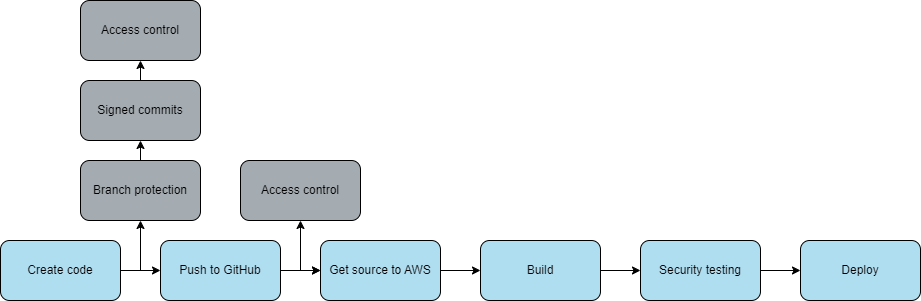
\includegraphics[width=0.8\columnwidth]{Images/pipeline7.png}
    \caption{Pipeline with implemented access control}
    \label{fig: Pipeline with implemented access control}
\end{figure}
 
\subsection{File Storage and Preservation}
To be able to maintain proper security of the pipeline, file storage, and preservation can be considered a large part of this. File storage and preservation help secure the pipeline over time, by doing regular backups of the data related to the pipeline. By maintaining redundant copies of critical data, the risk of data loss due to attacks or other security breaches can be minimized. 

Some other important aspect of file storage and preservation is access control, which should be restricted so one only has the necessary access. As a result, this can minimize the chances of data tampering or data theft.

\section{Security in maintenance}
Once the deployment is complete, the application is then transferred to the cloud environment in \acrlong{aws}. It is essential at this stage to keep the security up to date, to ensure that the application and data are protected. AWS offers a range of best practices organizations can follow to decrease risks associated with cloud computing and ensure that the  \acrshort{aws} environment is secure.

After the deployment is successful, it's essential to ensure that the infrastructure is secure and optimized for performance. Regular maintenance and updates are important to solve security issues and add new features to the system. It's also important to perform regular backups and disaster recovery testing to ensure that the data and applications are protected. 
Staying up-to-date with maintenance and testing can minimize downtime and improve system reliability. 

When the application is in the cloud environment, it is important to continuously monitor it. This is to identify any issues or potential threats. This includes monitoring for errors, performance issues, security vulnerabilities, and more. \acrshort{aws} offers specialized tools for this type of monitoring, like Amazon cloudwatch\footnote{Available at: https://aws.amazon.com/cloudwatch/} and AWS X-ray\footnote{Available at: https://aws.amazon.com/xray/}. 

Various security tests, such as security scans and penetration testing, should be performed during the development phases to identify potential vulnerabilities and address them before deployment. However, it is also essential to continue testing after deployment to ensure that any new vulnerabilities are identified and addressed as soon as possible. Regular security scans and penetration testing can significantly reduce the risk of exploitation. By conducting these tests regularly, the organization can keep track of any possible security problems and take proactive measures to mitigate them.

As a protective measure, the organization should set up a web application firewall like AWS WAF\footnote{Available at: https://aws.amazon.com/waf/}, to prevent malicious application attacks such as \gls{SQL-injection}, \gls{Cross-site scripting} and other attacks. AWS's WAF service offers a managed set of protective rules, allowing customized rules and access control lists based on the company's needs and risk models. This makes it possible to provide web application security with more customization and specificity. Securing an application against \gls{ddos} is an important additional step. AWS Shield\footnote{Available at: https://aws.amazon.com/shield/} is a service that an organization can utilize to achieve this. \cite{awsafterdep}

Security is an important aspect of the SDLC's maintenance phase, which begins after the application has been deployed. It is critical to keep up with regular maintenance and testing during this phase, as well as to take proactive measures to mitigate any issues that may arise. Organizations can identify and address potential security vulnerabilities in this manner before they become major issues. This is especially important when deploying applications to the cloud because the security environment can be complex and ever-changing. Best practices such as regular security audits, vulnerability scans, and the implementation of security patches can help to ensure that the application remains secure and protected against potential threats. Monitoring for unusual or suspicious activity can also aid in the detection and prevention of security breaches. Organizations can help to ensure the continued reliability and security of their AWS applications by prioritizing security throughout the maintenance phase.
\newpage
\section{Finished pipeline}
This is the finished pipeline after all security measures are included.

\vspace{2mm}
\begin{figure}[H]
    \centering
    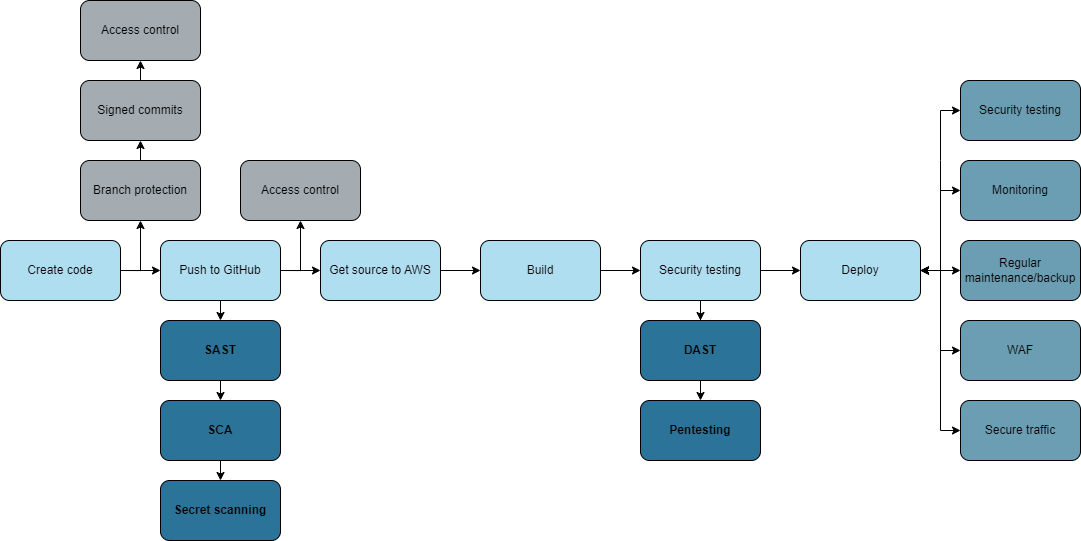
\includegraphics[width=0.8\columnwidth]{Images/pipeline9.png}
    \caption{Pipeline with all security measures implemented}
    \label{fig: Pipeline with all security measures implemented}
\end{figure}



